% Memoria del proyecto EHMbrAIn
% Compilar:  latexmk -pdf -outdir=build memoria.tex   (desde paper/memoria/)
%
% NOTA (repo público): el autor se mantiene anónimo en el repositorio.
% Rellenar \author localmente para la entrega académica; no commitear el nombre.

\documentclass[11pt,a4paper,oneside]{report}

\usepackage[utf8]{inputenc}
\usepackage[T1]{fontenc}
\usepackage[spanish,es-tabla]{babel}
\usepackage{lmodern}
\usepackage{microtype}
\usepackage{amsmath,amssymb}
\usepackage{siunitx}
\sisetup{output-decimal-marker={,},group-separator={\,}}
\usepackage{booktabs}
\usepackage{graphicx}
\graphicspath{{figuras/}}
\usepackage{csquotes}
\usepackage[style=numeric-comp,sorting=none,backend=biber]{biblatex}
\addbibresource{referencias.bib}
\usepackage[hidelinks]{hyperref}
\usepackage[spanish,capitalise]{cleveref}

\newcommand{\codigo}[1]{\texttt{#1}}

\title{\textbf{EHMbrAIn}\\[2mm]
  \large Monitorización de la salud de motores (EHM) basada en IA frente al
  enfoque tradicional: un banco de pruebas de \emph{Gas Path Analysis}
  sobre el CFM56-7B con verdad-terreno sintética}
\author{--- (anónimo en el repositorio público) ---}
\date{\today\\[2mm]\small Documento vivo: se actualiza con cada hito del proyecto.}

\begin{document}

\maketitle
\tableofcontents

\chapter{Introducción}
\label{cap:introduccion}

\section{Motivación}

La monitorización de la salud de motores aeronáuticos (\emph{Engine Health Monitoring}, EHM)
sostiene hoy decisiones de mantenimiento que mueven cifras enormes: un \emph{shop visit} de un
turbofan comercial cuesta del orden de millones de dólares, y una retirada no programada
multiplica ese coste por la disrupción operativa. La técnica de referencia desde los años setenta
es el \emph{Gas Path Analysis} (GPA)~\cite{Urban1975}: inferir el estado de salud de los
componentes del camino de gas (fan, compresores, turbinas) a partir de las medidas disponibles a
bordo (velocidades de rotor, temperatura de gases de escape, flujo de combustible, presiones).
Sobre el GPA se construyó toda una generación de sistemas industriales ---filtros de Kalman,
líneas base termodinámicas, reglas expertas de aislamiento~\cite{Volponi2014}--- que aquí
llamamos \emph{EHM tradicional}.

En la última década, el aprendizaje automático ha producido resultados llamativos en pronóstico
de vida útil remanente (RUL) sobre bancos de datos sintéticos como
C-MAPSS~\cite{Saxena2008} y N-CMAPSS~\cite{AriasChao2021}. Sin embargo, la literatura adolece de
un problema estructural: \textbf{casi nunca se compara la IA contra un enfoque tradicional
implementado con rigor}, sobre los mismos datos, con las mismas métricas y con el mismo esfuerzo
de ajuste. El resultado son comparaciones contra ``hombres de paja'' que impiden saber qué aporta
realmente la IA, cuándo y a qué coste.

\section{Objetivo}

Este trabajo construye un banco de pruebas reproducible en el que ambas familias de EHM
---tradicional y basada en IA--- observan \emph{exactamente los mismos datos} de una flota
sintética del turbofan CFM56-7B26 y se evalúan con \emph{exactamente las mismas métricas}. La
clave metodológica es que los datos sintéticos incorporan \textbf{verdad-terreno completa}: el
estado real de salud de cada componente (desviaciones de eficiencia y capacidad de flujo) en cada
vuelo. Esto, imposible con datos reales de aerolínea, permite medir no solo si un método detecta
o pronostica bien, sino si \emph{atribuye el daño al componente correcto} ---el talón de Aquiles
del GPA clásico (el fenómeno de \emph{smearing}) y la caja negra de la IA.

Al no existir ni un modelo de prestaciones del motor ni datos de degradación disponibles, el
proyecto construye ambos: un gemelo termodinámico del CFM56-7B26 en
pyCycle~\cite{Hendricks2019} calibrado contra datos públicos certificados
(\cref{cap:modelo}), y un generador de flota degradada con firmas de fallo físicas.

\section{Hipótesis}
\label{sec:hipotesis}

Las hipótesis se formalizan con umbrales cuantitativos \emph{antes} de ver los resultados del
conjunto de test (protocolo pre-registrado, \cref{sec:protocolo}). Todas se contrastan con test
de Wilcoxon pareado por motor, corrección de Holm ($\alpha = 0{,}05$) e intervalos bootstrap BCa.

\begin{table}[htbp]
  \centering\small
  \caption{Hipótesis del proyecto y criterios de confirmación.}
  \label{tab:hipotesis}
  \begin{tabular}{p{0.6cm}p{5.4cm}p{7.6cm}}
    \toprule
    ID & Hipótesis & Criterio de confirmación \\
    \midrule
    H1 & La IA detecta antes y con menos falsas alarmas que el \emph{trend monitoring} &
      \emph{lead time} mediano $\geq +20$\,\% y FPR $\leq 0{,}5\times$ frente al trending, a
      \emph{recall} fijo $0{,}9$; $p<0{,}05$ \\
    H2 & La IA aísla mejor fallos con firmas solapadas &
      $+10$ puntos de exactitud de aislamiento en el subconjunto ``confusable'' (firmas a
      $<15^{\circ}$ en el espacio de la ICM) frente a GPA-WLS; $p<0{,}05$ \\
    H3 & La IA pronostica mejor el RUL &
      mejora simultánea en RMSE y en el \emph{score} asimétrico NASA PHM08; $p<0{,}05$ \\
    H4 & El híbrido \emph{physics-informed} domina con pocos datos &
      RMSE de RUL $\leq$ IA pura con el 100\,\% del entrenamiento y estrictamente mejor con el
      10\,\% y el 25\,\%; $p<0{,}05$ \\
    H5 & Los intervalos \emph{conformal} calibran mejor que la covarianza del Kalman &
      menor $|$cobertura empírica $-$ 0{,}9$|$ con anchura media no peor que $+20$\,\% \\
    \bottomrule
  \end{tabular}
\end{table}

La refutación de cualquier hipótesis es también un resultado publicable: el pre-registro la hace
creíble. Queda prohibido reformular hipótesis tras la etiqueta \codigo{prereg-v1} del
repositorio.

\section{Contribuciones}
\label{sec:contribuciones}

\begin{enumerate}
  \item[\textbf{C1.}] \textbf{SynCFM56}: primer conjunto de datos sintético público de GPA sobre
    un motor comercial concreto (CFM56-7B26), con verdad-terreno de parámetros de salud por
    vuelo y formato de \emph{snapshots} tipo ACARS (informe de despegue + informe de crucero por
    vuelo), más realista que las series continuas de C-MAPSS.
  \item[\textbf{C2.}] Comparación cabeza a cabeza con \textbf{protocolo pre-registrado} e igual
    presupuesto de ajuste (mismo número de \emph{trials} de Optuna) para ambas familias.
  \item[\textbf{C3.}] Híbrido \emph{physics-informed} con tres mecanismos ablacionados por
    separado: residuos contra el gemelo digital, pérdidas con restricciones físicas y
    \emph{stacking} GPA$\rightarrow$ML.
  \item[\textbf{C4.}] Cuantificación de incertidumbre comparada: intervalos de RUL por
    \emph{conformal prediction} frente a la covarianza del filtro de Kalman.
  \item[\textbf{C5.}] \textbf{Physics-Consistency Score (PCS)}: métrica nueva de explicabilidad
    que proyecta las atribuciones SHAP al espacio físico de parámetros de salud vía la matriz de
    coeficientes de influencia.
  \item[\textbf{C6.}] Mapa de determinabilidad: ablación sensores $\times$ ruido $\times$ tamaño
    de datos que muestra \emph{cuándo} gana cada enfoque.
  \item[\textbf{C7.}] Validación \emph{sim-to-real}: la metodología completa se re-ejecuta sobre
    N-CMAPSS para comprobar que el \emph{ranking} de métodos no es un artefacto del simulador
    propio.
\end{enumerate}

\section{Estructura del documento}

El \cref{cap:fundamentos} fija los fundamentos: el motor, la formulación del GPA y la física de
la degradación. El \cref{cap:metodologia} describe la arquitectura del banco de pruebas y las
salvaguardas metodológicas. El \cref{cap:modelo} documenta el gemelo termodinámico del
CFM56-7B26 y su calibración contra datos certificados ---el trabajo completado hasta la fecha---
con las evidencias cuantitativas del proceso. El \cref{cap:trabajo-en-curso} resume las fases
restantes y sus criterios de aceptación.

\chapter{Fundamentos}
\label{cap:fundamentos}

\section{El motor: CFM56-7B26}
\label{sec:motor}

El CFM56-7B (CFM International, consorcio Safran--GE) propulsa la familia Boeing 737NG y es uno
de los motores comerciales más extendidos de la historia, lo que garantiza abundancia de datos
públicos de tipo. Se elige la variante \textbf{-7B26} (\SI{117}{\kilo\newton} de empuje de
despegue, Boeing 737-800) por ser la más común. Según su hoja de datos de certificado de tipo
(TCDS EASA E.004, ed.~07~\cite{EASA2023}), es un turbofan de doble rotor y alta relación de
derivación: fan de una etapa, compresor de baja (\emph{booster}) de 3 etapas, compresor de alta
(HPC) de 9 etapas, cámara de combustión anular, turbina de alta (HPT) de 1 etapa y turbina de
baja (LPT) de 4 etapas, con control digital FADEC de doble canal. El parámetro primario de
empuje es N1 (velocidad del rotor de baja), no EPR.

\begin{table}[htbp]
  \centering\small
  \caption{Datos certificados del CFM56-7B26 empleados como contrato de calibración. Fuentes:
  TCDS EASA E.004 ed.~07~\cite{EASA2023} y banco de datos de emisiones OACI, ed.~03/2026, UID
  3CM033~\cite{ICAO2026}.}
  \label{tab:tcds}
  \begin{tabular}{llll}
    \toprule
    Magnitud & Valor & Fuente & Estado \\
    \midrule
    Empuje de despegue & \SI{11699}{\deca\newton} (= \SI{116.99}{\kilo\newton}) & TCDS & verificado \\
    Empuje máximo continuo & \SI{11521}{\deca\newton} & TCDS & verificado \\
    N1 límite (104\,\%) & \SI{5382}{rpm} $\Rightarrow$ 100\,\% = \SI{5175}{rpm} & TCDS & verificado \\
    N2 límite (105\,\%) & \SI{15183}{rpm} $\Rightarrow$ 100\,\% = \SI{14460}{rpm} & TCDS & verificado \\
    EGT máx.\ despegue / continuo & \SI{950}{\degreeCelsius} / \SI{925}{\degreeCelsius} (mostrada) & TCDS & verificado \\
    Peso en seco & \SI{2386}{\kilo\gram} & TCDS & verificado \\
    Relación de derivación & 5{,}1 & EEDB & verificado \\
    Relación de presiones (SLS, nominal) & 27{,}61 & EEDB & verificado \\
    $W_f$ a 100/85/30/7\,\% $F_{00}$ & 1{,}221 / 0{,}999 / 0{,}338 / 0{,}113 \si{\kilo\gram\per\second} & EEDB & verificado \\
    \bottomrule
  \end{tabular}
\end{table}

Dos matices del TCDS resultan relevantes para el modelado y suelen pasarse por alto:
\begin{itemize}
  \item La EGT certificada se mide en la estación \textbf{T49.5} (tobera de la segunda etapa de
    la LPT), no en la salida de la HPT; y el valor \emph{mostrado} en cabina añade una función
    \emph{shunt} de $+\SI{30}{\degreeCelsius}$ (motores SAC, activa por encima de \SI{8500}{rpm} de
    N2) más un \emph{trim} dependiente del modelo (nulo para el -7B26).
  \item Los límites de sangrado están tabulados por estación de extracción (5.ª y 9.ª etapa del
    HPC) y régimen; a régimen nominal el sangrado de 9.ª etapa se limita al 7\,\% del flujo
    primario.
\end{itemize}

\section{Estaciones y parámetros corregidos}
\label{sec:estaciones}

Se adopta la numeración SAE ARP755A~\cite{SAE755}: 2 entrada del fan; 21 salida del fan; 25
entrada del HPC; 3 salida del HPC; 4 salida de cámara; 45 salida de la HPT; 5 salida de la LPT.
El rotor de baja (N1) une fan, \emph{booster} y LPT; el de alta (N2), HPC y HPT.

Para comparar vuelos en condiciones distintas, las medidas se corrigen a condiciones ISA a nivel
del mar con $\theta = T_{t2}/\SI{288.15}{\kelvin}$ y $\delta = P_{t2}/\SI{101.325}{\kilo\pascal}$:
\begin{equation}
  N_{\mathrm{corr}} = \frac{N}{\sqrt{\theta}}, \qquad
  W_{f,\mathrm{corr}} = \frac{W_f}{\delta\,\theta^{a}}, \qquad
  \mathrm{EGT}_{\mathrm{corr}} = \frac{\mathrm{EGT}}{\theta},
\end{equation}
donde el exponente $a$ (habitualmente $0{,}5$--$0{,}7$) no se toma de tablas genéricas sino que
se ajustará por regresión sobre barridos del propio modelo termodinámico, eliminando una fuente
clásica de error sistemático en las líneas base.

\section{Formulación del \emph{Gas Path Analysis}}
\label{sec:gpa}

El estado de salud del camino de gas se describe con el vector de desviaciones respecto a motor
nuevo
\begin{equation}
  \mathbf{x} = \left[\Delta\eta_{\mathrm{fan}}, \Delta\Gamma_{\mathrm{fan}},
  \Delta\eta_{\mathrm{LPC}}, \Delta\Gamma_{\mathrm{LPC}},
  \Delta\eta_{\mathrm{HPC}}, \Delta\Gamma_{\mathrm{HPC}},
  \Delta\eta_{\mathrm{HPT}}, \Delta\Gamma_{\mathrm{HPT}},
  \Delta\eta_{\mathrm{LPT}}, \Delta\Gamma_{\mathrm{LPT}}\right]^{\mathsf T},
\end{equation}
donde $\Delta\eta$ es la desviación relativa de eficiencia isentrópica y $\Delta\Gamma$ la de
capacidad de flujo corregida de cada turbomáquina. Las medidas disponibles se expresan como
desviaciones $\Delta\mathbf{z}$ de los parámetros corregidos respecto a la línea base en el
mismo punto de operación $\mathbf{u}$ (altitud, Mach, N1, $\Delta T_{\mathrm{ISA}}$, sangrado).
El modelo lineal local es
\begin{equation}
  \Delta\mathbf{z} = \mathbf{H}(\mathbf{u})\,\mathbf{x} + \mathbf{S}\,\mathbf{b} + \mathbf{v},
  \qquad \mathbf{v}\sim\mathcal{N}(\mathbf{0},\mathbf{R}),
  \label{eq:gpa-lineal}
\end{equation}
con $\mathbf{H}$ la \emph{matriz de coeficientes de influencia} (ICM), jacobiano
$\partial\mathbf{z}/\partial\mathbf{x}$ evaluado en $\mathbf{u}$ y obtenido por diferencias
centrales sobre el modelo termodinámico; $\mathbf{b}$ los sesgos de sensor y $\mathbf{R}$ la
covarianza del ruido de medida.

\paragraph{Estimación WLS.} Con 4 medidas de cabina (N1, N2, EGT, $W_f$) y 10 incógnitas el
sistema es infra-determinado ($\operatorname{rango}(\mathbf{H})\leq 4$), por lo que la solución
de mínimos cuadrados ponderados exige regularización con una prior $\mathbf{P}_0$ de magnitudes
de deterioro esperables:
\begin{equation}
  \hat{\mathbf{x}} = \left(\mathbf{H}^{\mathsf T}\mathbf{R}^{-1}\mathbf{H}
  + \lambda\,\mathbf{P}_0^{-1}\right)^{-1}\mathbf{H}^{\mathsf T}\mathbf{R}^{-1}\Delta\mathbf{z}.
  \label{eq:wls}
\end{equation}

\paragraph{Seguimiento con filtro de Kalman.} El deterioro evoluciona lentamente, lo que
justifica un modelo de paseo aleatorio:
\begin{equation}
  \mathbf{x}_k = \mathbf{x}_{k-1} + \mathbf{w}_k, \quad \mathbf{w}\sim\mathcal{N}(\mathbf{0},\mathbf{Q});
  \qquad
  \mathbf{z}_k = \mathbf{H}(\mathbf{u}_k)\,\mathbf{x}_k + \mathbf{v}_k,
  \label{eq:kalman}
\end{equation}
con $\mathbf{Q}$ calibrada a las tasas de degradación y estado aumentable con sesgos de sensor
\cite{Volponi2014}. En los eventos registrados de lavado de compresor se reinicia la parte
recuperable del estado.

\paragraph{\emph{Smearing} y observabilidad.} Cuando $\mathbf{H}$ está mal condicionada, el
ruido proyecta un fallo concentrado en un solo componente sobre varios: es el fenómeno de
\emph{smearing}, debilidad clásica del GPA lineal~\cite{Li2002}. El análisis SVD de la ICM
(rango, número de condición, ángulos entre firmas de fallo) cuantifica esta debilidad y define
el subconjunto ``confusable'' usado por la hipótesis H2: pares de fallos cuyas firmas forman un
ángulo inferior a $15^{\circ}$.

\section{Física de la degradación}
\label{sec:degradacion}

\begin{table}[htbp]
  \centering\small
  \caption{Mecanismos de degradación modelados y efectos típicos según la
  literatura~\cite{Diakunchak1992,Kurz2012}.}
  \label{tab:degradacion}
  \begin{tabular}{p{3.2cm}p{2.2cm}p{3.6cm}p{2.6cm}p{1.6cm}}
    \toprule
    Mecanismo & Componente & Efecto típico & Perfil temporal & Recuperable \\
    \midrule
    \emph{Fouling} & fan/LPC/HPC & $\Delta\Gamma$ $-1$\ldots$-4$\,\%; $\Delta\eta$ $-0{,}5$\ldots$-2{,}5$\,\% & exponencial saturante & lavado (30--70\,\%) \\
    Erosión & compresores & $\Delta\eta$ $-0{,}5$\ldots$-1{,}5$\,\% & lineal lento & no \\
    Holgura de punta & HPC/HPT & $\Delta\eta$ $-0{,}5$\ldots$-1{,}5$\,\% & rápido inicial, luego lento & no \\
    Deterioro sección caliente & HPT & $\Delta\eta$ $-1$\ldots$-3$\,\%; $\Delta\Gamma$ $+1$\ldots$+2$\,\% & lineal/acelerado & no \\
    FOD & fan/HPC & escalón $\Delta\eta$ $-0{,}5$\ldots$-2$\,\% & escalón (Poisson) & no \\
    Deriva de sensor & cualquier sonda & p.\ ej.\ EGT $+1$\ldots$+5$~\si{\degreeCelsius}/1000 ciclos & rampa & recalibración \\
    \bottomrule
  \end{tabular}
\end{table}

El efecto agregado observable es la erosión del \emph{margen de EGT} (distancia entre la EGT en
despegue de día caliente y su límite certificado), desde \SI{70}{}--\SI{100}{\degreeCelsius} en motor
nuevo hasta cero al final de la vida útil en ala, con el patrón característico ``rápido al
principio, lento después, dientes de sierra por lavados''. La \cref{tab:degradacion} resume los
mecanismos, sus firmas y sus perfiles temporales; sus magnitudes parametrizan el generador de
flota sintética de la fase F2.

\chapter{Metodología y arquitectura del banco de pruebas}
\label{cap:metodologia}

\section{Arquitectura general}

El banco de pruebas se organiza en seis fases encadenadas, cada una cerrada por un hito
(\emph{gate}) con criterio de aceptación medible:

\begin{enumerate}
  \item[\textbf{F1.}] \textbf{Gemelo termodinámico} del CFM56-7B26 en pyCycle: ciclo de diseño,
    fuera de diseño, \emph{decks} de línea base sobre la envolvente y matriz de coeficientes de
    influencia (ICM). \emph{Gate} H1: error $\leq 3$\,\% frente a los datos certificados en los
    puntos ancla.
  \item[\textbf{F2.}] \textbf{Generador de flota sintética} (SynCFM56): trayectorias de salud por
    mecanismo, flota jerárquica de $\sim$100 motores \emph{run-to-failure}, modelo de sensores
    (ruido, sesgo, cuantización, huecos) y \emph{snapshots} tipo ACARS con verdad-terreno.
    \emph{Gate} H2: dataset auditado, sin fuga entre particiones, con dificultad verificada.
  \item[\textbf{F3.}] \textbf{EHM tradicional} de referencia: línea base y desviaciones
    suavizadas, \emph{trending} con reglas de persistencia, GPA-WLS
    (\cref{eq:wls}), Kalman-GPA (\cref{eq:kalman}), aislamiento por reglas expertas y RUL por
    extrapolación robusta del margen de EGT. \emph{Gate} H3: métricas completas sobre test.
  \item[\textbf{F4.}] \textbf{EHM con IA}: detección de anomalías (autoencoder, Isolation
    Forest), diagnóstico multiclase (XGBoost, redes), pronóstico de RUL (LSTM/TCN/Transformer),
    híbrido \emph{physics-informed}, incertidumbre \emph{conformal} y explicabilidad
    física (PCS). \emph{Gate} H4.
  \item[\textbf{F5.}] \textbf{Evaluación comparativa pre-registrada}: métricas comunes,
    contrastes estadísticos, ablaciones y validación \emph{sim-to-real} en N-CMAPSS.
    \emph{Gate} H5.
  \item[\textbf{F6.}] Casos de estudio, \emph{dashboard} y redacción. \emph{Gate} H6.
\end{enumerate}

\section{Salvaguardas metodológicas}
\label{sec:protocolo}

La credibilidad de una comparación IA-contra-tradicional depende de eliminar los sesgos que
plagan la literatura. Se adoptan cuatro salvaguardas:

\begin{description}
  \item[Pre-registro.] Hipótesis (\cref{tab:hipotesis}), métricas, particiones (con \emph{hash}
    de los ficheros), contrastes y regla de parada se congelan en el repositorio con una
    etiqueta de git (\codigo{prereg-v1}) \emph{antes} de evaluar sobre el conjunto de test.
  \item[Presupuesto de ajuste simétrico.] Los hiperparámetros del pipeline tradicional
    (umbrales, $\lambda$, $\mathbf{Q}$, ventanas) y de cada familia de IA se ajustan con el
    mismo número de \emph{trials} de Optuna, usando solo entrenamiento y validación.
  \item[Partición por motor.] Ningún motor aparece en más de una partición
    (70/10/20 motores en train/val/test), con auditoría automática anti-fuga en integración
    continua.
  \item[Baseline fuerte.] El pipeline tradicional se implementa con el mismo cuidado que la IA,
    documentando cada regla con su justificación física; el \emph{smearing} se mide contra la
    verdad-terreno, no se asume.
\end{description}

\section{Reproducibilidad e infraestructura}
\label{sec:reproducibilidad}

Todo el proyecto es un repositorio público\footnote{\url{https://github.com/cedarcreeks/EHMbrAIn}}
con entorno reproducible: Python~3.11 gestionado con \codigo{uv} y versiones bloqueadas
(\codigo{uv.lock}); pyCycle~4.4 sobre OpenMDAO~\cite{Gray2019}; configuraciones declarativas en
YAML; y pruebas automatizadas (pytest) ejecutadas en integración continua en cada cambio. Los
datos y experimentos de fases posteriores se versionarán con DVC y MLflow respectivamente.

Dos decisiones concretas ilustran el estándar de rigor perseguido:

\begin{itemize}
  \item \textbf{Contrato de calibración versionado.} Los objetivos numéricos del modelo
    (\cref{tab:tcds}) viven en un único fichero
    (\codigo{conf/cfm56\_7b\_targets.yaml}) con valor, tolerancia, fuente y estado
    (\codigo{VERIFIED}/\codigo{TO\_VERIFY}) por entrada. Ese fichero lo leen tanto los
    ejecutores del modelo como las pruebas: un cambio de objetivo es un cambio visible en el
    control de versiones, nunca una edición silenciosa.
  \item \textbf{Pruebas canario de dependencias.} Durante la puesta en marcha se detectó una
    incompatibilidad entre pyCycle~4.4 y numpy~$\geq 2$ (error en el cálculo termodinámico
    tabular). Se fijó \codigo{numpy<2} y se dejó una prueba de humo que ejecuta un ciclo
    completo en cada ejecución de CI, de modo que cualquier actualización de dependencias que
    rompa el solver falle de forma visible e inmediata.
  \item \textbf{Cifras autogeneradas.} Todas las figuras y tablas de resultados de este
    documento las genera un script (\codigo{scripts/make\_memoria\_assets.py}) que resuelve el
    modelo y escribe directamente los PDF y los ficheros \LaTeX{}
    (\codigo{paper/memoria/tablas/*.tex}), junto con un \codigo{assets.json} de
    trazabilidad. Ningún número de resultados se copia a mano.
\end{itemize}

\section{Métricas de comparación}

Ambas familias se evalúan con métricas idénticas: para detección, \emph{lead time}, tasa de
falsas alarmas por mil vuelos, F1 y PR-AUC; para aislamiento, exactitud top-1/top-2, macro-F1,
índice de \emph{smearing} (fracción de $\|\hat{\mathbf{x}}\|_1$ asignada a componentes sanos) y
PCS; para la estimación de salud, RMSE de $\hat{\mathbf{x}}$ frente a la verdad-terreno; para el
RUL, RMSE, MAE, \emph{score} NASA PHM08
\begin{equation}
  S=\sum_i s_i,\qquad
  s_i = \begin{cases} e^{-d_i/13}-1 & d_i<0\\ e^{d_i/10}-1 & d_i\geq 0\end{cases},
  \qquad d_i = \widehat{\mathrm{RUL}}_i - \mathrm{RUL}_i,
\end{equation}
exactitud $\alpha$--$\lambda$ y horizonte de pronóstico; y para la incertidumbre, cobertura
empírica frente a nominal y anchura media de los intervalos.

\chapter{Gemelo termodinámico del CFM56-7B26}
\label{cap:modelo}

Este capítulo documenta el trabajo completado de la fase F1: el modelo de prestaciones del
CFM56-7B26 en pyCycle~\cite{Hendricks2019}, su punto de diseño (WP1.1) y su calibración fuera de
diseño contra datos medidos certificados (WP1.2). Todas las cifras de resultados provienen del
script de generación de evidencias (\cref{sec:reproducibilidad}).

\section{Estrategia: adaptar, no construir desde cero}
\label{sec:morph}

pyCycle distribuye un ejemplo validado de turbofan de alta derivación de doble rotor y flujo
separado con refrigeración de turbinas (\codigo{high\_bypass\_turbofan.py}), con el grafo de
elementos, la red de sangrados, los balances de ejes y el solver fuera de diseño ya operativos.
Construir el CFM56 desde un fichero en blanco obliga a re-derivar todo ese cableado y suele
morir en divergencias del método de Newton. En su lugar se adopta un protocolo de
\emph{morphing}: el ejemplo se toma como estado conocido-bueno (y se conserva en el repositorio
como referencia de regresión) y se re-orienta hacia el CFM56-7B26 cambiando \textbf{como máximo
tres parámetros por paso}, exigiendo convergencia en cada paso antes del siguiente. Cada paso
convergido es un \emph{commit}; si un paso diverge, se bisecta el cambio.

Las decisiones de diseño se fijaron por escrito \emph{antes} de codificar
(\codigo{docs/f1-model-spec.md}): variante -7B26; termodinámica tabular con verificación cruzada
CEA; punto de diseño en crucero M\,0,78 / \SI{35000}{ft} / ISA; mapas genéricos de pyCycle
escalados (no existen mapas públicos del CFM56) con extrapolación controlada; potencia fijada
por N1 corregida en fuera de diseño (el -7B es un motor regulado por N1); unidades nativas de
pyCycle en el interior del modelo y SI solo en la frontera; y una tabla de modos de fallo del
solver con su contramedida prevista, que resultó profética (\cref{sec:idle}).

\section{Punto de diseño (WP1.1)}
\label{sec:diseno}

El grafo del ciclo comprende: condiciones de vuelo, entrada, fan, divisor de flujo,
\emph{booster}, HPC con tres puertos de sangrado (refrigeración de vano y álabe de HPT y
sangrado de cliente), sangrado post-compresor para la LPT, cámara, HPT y LPT refrigeradas,
conductos con pérdidas de presión, toberas convergentes de núcleo y derivación, dos ejes y
extracción de potencia de accesorios (\SI{250}{hp} en el eje de alta). En el punto de diseño,
cuatro balances implícitos determinan el ciclo: el gasto $W$ ajusta el empuje objetivo; el
dosado FAR ajusta $T_{t4}$; y las relaciones de expansión de HPT y LPT anulan la potencia neta
de cada eje.

\begin{table}[htbp]
  \centering\small
  \caption{Resultados del punto de diseño (M\,0,78, \SI{35000}{ft}, ISA). Tabla autogenerada
  desde el modelo.}
  \label{tab:diseno}
  % AUTOGENERADO por scripts/make_memoria_assets.py — NO editar a mano
\begin{tabular}{ll}
\toprule
Magnitud & Valor en el punto de diseño \\
\midrule
  Empuje neto $F_n$ & \SI{24.38}{\kilo\newton} (\num{5480} lbf) \\
  TSFC & \num{0.6214} lb/(lbf$\cdot$h) \\
  Relación de derivación (BPR) & \num{5.10} \\
  Relación de compresión global (OPR) & \num{30.03} \\
  $T_{t4}$ & \SI{1587}{\kelvin} (\num{2857} °R) \\
  Gasto másico $W$ & \SI{142.0}{\kilo\gram\per\second} \\
  Dosado FAR & \num{0.0251} \\
  Relación de expansión HPT & \num{3.586} \\
  Relación de expansión LPT & \num{4.288} \\
  Fracción total de refrigeración/sangrado & \num{0.239} \\
\bottomrule
\end{tabular}

\end{table}

\begin{table}[htbp]
  \centering\small
  \caption{Condiciones totales por estación en el punto de diseño. Tabla autogenerada.}
  \label{tab:estaciones}
  % AUTOGENERADO por scripts/make_memoria_assets.py — NO editar a mano
\begin{tabular}{llrr}
\toprule
Estación & Posición & $P_t$ [bar] & $T_t$ [K] \\
\midrule
  2 & Entrada fan & 0.358 & 245.5 \\
  21 & Salida fan & 0.603 & 289.5 \\
  25 & Entrada HPC & 1.149 & 354.2 \\
  3 & Salida HPC & 10.739 & 703.9 \\
  4 & Salida cámara & 10.159 & 1587.2 \\
  45 & Salida HPT & 2.833 & 1141.6 \\
  5 & Salida LPT & 0.657 & 806.3 \\
\bottomrule
\end{tabular}

\end{table}

\begin{figure}[htbp]
  \centering
  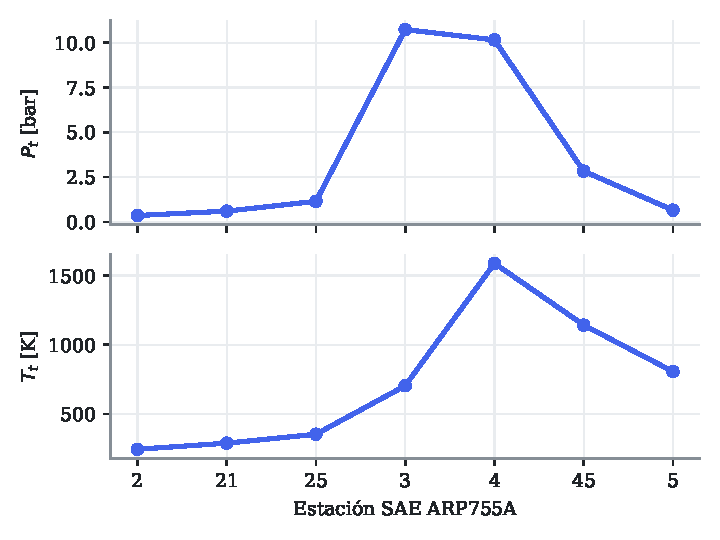
\includegraphics[width=0.72\textwidth]{estaciones_diseno}
  \caption{Evolución de presión y temperatura totales a lo largo del camino de gas en el punto
  de diseño. La compresión culmina en la estación 3 ($\sim$\SI{11}{bar},
  \cref{tab:estaciones}), la adición de calor en la 4 y la extracción de trabajo en 45 y 5.}
  \label{fig:estaciones}
\end{figure}

El punto de diseño converge con residuo de Newton inferior a $10^{-6}$ y satisface las cinco
ventanas de aceptación definidas a priori: BPR $5{,}10\pm0{,}2$ (objetivo EEDB), OPR en ventana,
$T_{t4}$ en banda plausible, fracción total de refrigeración y sangrado en 18--25\,\% del flujo
de núcleo, y empuje exacto al objetivo (\cref{tab:diseno}). El TSFC resultante
($\approx0{,}62$~lb/(lbf$\cdot$h)) queda a menos del 2\,\% del valor de crucero citado
públicamente para este motor, sin haberse usado como objetivo de ajuste.

\section{Calibración contra datos medidos (WP1.2)}
\label{sec:calibracion}

\subsection{Fuentes de datos y filosofía}

La calibración fuera de diseño usa exclusivamente \textbf{datos medidos y certificados}
(\cref{tab:tcds}): la TCDS aporta límites y empujes nominales, y el banco de emisiones OACI
aporta los flujos de combustible medidos en banco a nivel del mar en los cuatro reglajes del
ciclo aterrizaje-despegue (100, 85, 30 y 7\,\% del empuje nominal $F_{00}$), además de la
relación de presiones del motor al régimen nominal (27{,}61). Estos cuatro puntos ---ignorados
por la mayoría de trabajos académicos--- constituyen anclas de calibración gratuitas, trazables
y de calidad de certificación.

Los puntos ancla se resuelven \emph{a empuje impuesto} (el dosado equilibra
$F_n = \mathrm{PC}\cdot F_{00}$): así el flujo de combustible del modelo es una
\textbf{predicción} genuina que se confronta con la medida del EEDB, no un ajuste.

\subsection{Iteraciones de calibración}

La primera ejecución (modelo recién adaptado del ejemplo, sin calibrar a los datos SLS) predijo
el flujo de combustible de despegue con un error de $-2{,}1$\,\%, pero presentó dos defectos
cuantitativos:

\begin{enumerate}
  \item \textbf{N2 al empuje nominal por encima de la línea roja}: \SI{15311}{rpm} frente al
    límite certificado de \SI{15183}{rpm}. Causa: la referencia de velocidad con la que se
    escala el mapa genérico del HPC. Corrección: referencia de diseño del eje de alta de
    \SI{14324}{} a \SI{13940}{rpm}, con lo que el régimen nominal queda en \SI{14915}{rpm}
    ($\approx103$\,\%), dentro del límite.
  \item \textbf{OPR de despegue $28{,}99$ frente al valor medido $27{,}61$} ($+5{,}0$\,\%).
    Corrección: relación de compresión del HPC en el punto de diseño de $9{,}81$ a $9{,}35$; el
    dato medido prevalece sobre la estimación derivada inicial, y el OPR de crucero pasa a ser
    una consecuencia ($\approx30$).
\end{enumerate}

\begin{table}[htbp]
  \centering\small
  \caption{Anclas SLS frente a las medidas del banco OACI tras la calibración. $W_f$~mod.\ es la
  predicción del modelo a empuje impuesto. Tabla autogenerada.}
  \label{tab:anclas}
  % AUTOGENERADO por scripts/make_memoria_assets.py — NO editar a mano
\begin{tabular}{lrrrrrrc}
\toprule
Ancla & \%$F_{00}$ & $F_n$ [kN] & $W_f$ mod. & $W_f$ EEDB & error [\%] & tol. [\%] & gate \\
\midrule
  A2 Takeoff & 100 & 117.0 & 1.204 & 1.221 & -1.40 & \num{3.0} & \checkmark \\
  A3 Climbout & 85 & 99.4 & 0.977 & 0.999 & -2.23 & \num{3.0} & \checkmark \\
  A4 Approach & 30 & 35.1 & 0.328 & 0.338 & -3.08 & \num{5.0} & \checkmark \\
  A5 Idle & 7 & 8.2 & 0.125 & 0.113 & +10.57 & \num{5.0} & --- \\
\bottomrule
\end{tabular}

\end{table}

\begin{figure}[htbp]
  \centering
  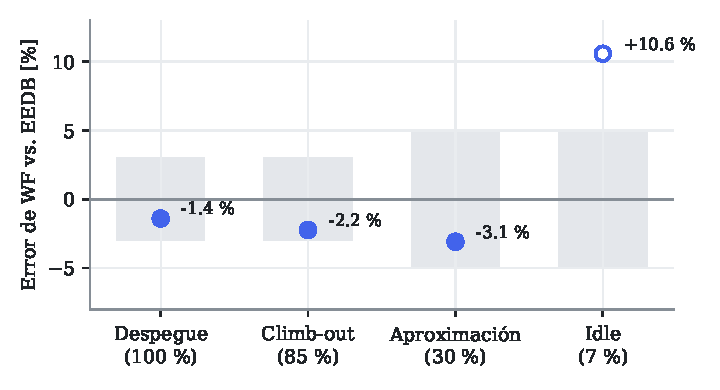
\includegraphics[width=0.7\textwidth]{errores_anclas}
  \caption{Error de la predicción de flujo de combustible en cada ancla frente a la medida del
  EEDB. Las bandas grises son las tolerancias del contrato ($\pm3$\,\% en despegue y
  \emph{climb-out}, $\pm5$\,\% en aproximación e idle); el punto hueco (idle) converge pero
  queda fuera de tolerancia y se reporta sin bloquear el hito (\cref{sec:idle}).}
  \label{fig:errores-anclas}
\end{figure}

\begin{figure}[htbp]
  \centering
  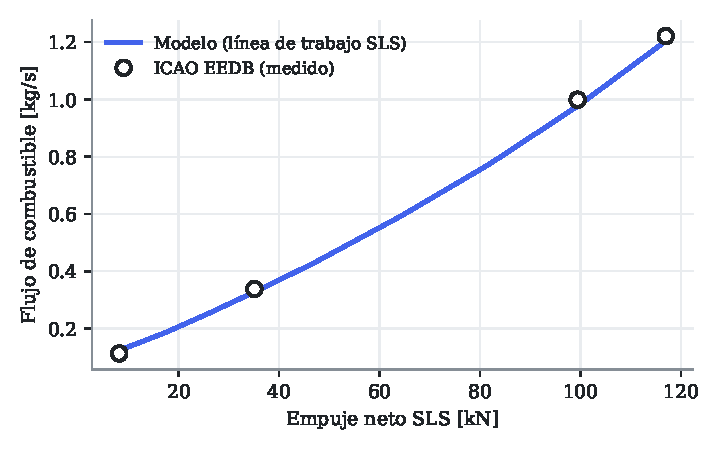
\includegraphics[width=0.7\textwidth]{linea_trabajo_sls}
  \caption{Línea de trabajo del modelo a nivel del mar estático (barrido continuo de reglaje de
  empuje) frente a los cuatro puntos medidos del banco OACI. La curvatura a baja potencia
  refleja el deterioro del rendimiento con mapas genéricos lejos del punto de escalado.}
  \label{fig:linea-trabajo}
\end{figure}

Tras ambas correcciones (\cref{tab:anclas,fig:errores-anclas,fig:linea-trabajo}), las tres
anclas con \emph{gate} cumplen sus tolerancias: despegue $-1{,}40$\,\% de error en $W_f$ con OPR
a $+0{,}3$\,\% del medido y ambos regímenes dentro de las líneas rojas; \emph{climb-out}
$-2{,}23$\,\%; aproximación $-3{,}08$\,\%.

\subsection{Convergencia en idle: diagnóstico y solución}
\label{sec:idle}

El punto de idle (7\,\% de $F_{00}$, estático) diverge sistemáticamente desde arranque en frío:
con relaciones de expansión de tobera próximas a la unidad, el subsolver de presión estática de
las toberas rebota contra su cota inferior y el Newton global no encuentra dirección de
descenso. Peor aún, el intento fallido deja los estados internos del punto (estaciones de flujo,
posiciones de mapa) corrompidos, de modo que re-sembrar solo los balances no lo rescata: fue
necesario que el punto de idle \emph{nunca} arranque en frío en su reglaje final. La solución
---prevista como contramedida genérica en la especificación--- es una \textbf{continuación en
potencia}: el punto arranca al 30\,\% de $F_{00}$ (donde converge de frío, igual que el ancla de
aproximación) y desciende en caliente por la secuencia $0{,}30 \rightarrow 0{,}20 \rightarrow
0{,}14 \rightarrow 0{,}10 \rightarrow 0{,}08 \rightarrow 0{,}07$, re-resolviendo el problema en
cada paso. Esta lógica queda encapsulada en la librería (\codigo{solve\_anchors()}) y cubierta
por las pruebas.

Con la continuación, el idle converge y predice $W_f$ con $+10{,}6$\,\% de error. Es territorio
de extrapolación profunda de los mapas genéricos (la forma velocidad-flujo a muy baja potencia
no es la del compresor real), una limitación conocida del enfoque; el ancla se \textbf{reporta
pero no bloquea} el hito H1, decisión documentada en el contrato de calibración
(\codigo{gated:~false}).

\section{Limitaciones declaradas}
\label{sec:limitaciones}

El modelo es \emph{representativo}, no certificable, y sus límites se declaran para su cita en
los capítulos de resultados: (i) sin transitorios ---solo estados estacionarios---; (ii)
geometría variable (VBV/VSV) implícita en los mapas, no modelada; (iii) sin correcciones de
Reynolds ni humedad; (iv) las etiquetas absolutas de N1/N2 son aproximadas por construcción
(formas de mapa genéricas), aunque respetan las líneas rojas certificadas en el punto nominal;
(v) la EGT del modelo es la temperatura de salida de la HPT (estación 45), un \emph{proxy}
coherente ---idéntico para la verdad-terreno y para ambos pipelines de EHM--- de la T49.5
certificada, cuyo valor mostrado además incorpora las funciones \emph{shunt} y \emph{trim}
descritas en \cref{sec:motor}; y (vi) el error de idle citado arriba. Ninguna de estas
limitaciones afecta a la validez de la comparación IA-contra-tradicional, que se apoya en la
estructura de sensibilidades del modelo (la ICM), no en sus valores absolutos.

\section{Verificación automatizada}

El estado del capítulo queda blindado por pruebas: convergencia y ventanas del punto de diseño;
convergencia de las cuatro anclas con la continuación de idle; tolerancias de $W_f$ y OPR en las
anclas con \emph{gate}; líneas rojas de N1/N2 al empuje nominal; y la prueba de humo del entorno
pyCycle. Nueve pruebas en verde en integración continua en el momento de escribir este
capítulo.

\chapter{Trabajo en curso y planificación}
\label{cap:trabajo-en-curso}

\section{Cierre de la fase F1}

Para cerrar el hito H1 restan dos paquetes de trabajo:

\begin{description}
  \item[WP1.3 — \emph{Decks} de línea base.] Barrido del modelo sobre la envolvente operativa
    (altitud $\times$ Mach $\times$ reglaje $\times$ $\Delta T_{\mathrm{ISA}}$ $\times$
    sangrado) y empaquetado de un interpolador validado por \emph{leave-one-out}
    (error de interpolación $<0{,}1$\,\%). Este interpolador es la línea base contra la que
    ambos pipelines de EHM calcularán desviaciones.
  \item[WP1.4 — Matriz de coeficientes de influencia.] Diferencias centrales ($\pm0{,}5$\,\%)
    sobre los diez parámetros de salud en una sub-rejilla de puntos de operación; análisis SVD
    (rango, número de condición, ángulos entre firmas) que define el subconjunto ``confusable''
    de la hipótesis H2; y pruebas físicas automáticas de signos (p.\ ej.\
    $\Delta\eta_{\mathrm{HPT}}\downarrow \Rightarrow \mathrm{EGT}\uparrow, W_f\uparrow$).
    Verificación cruzada de la termodinámica tabular contra CEA en los puntos ancla.
\end{description}

\section{Fases siguientes}

\begin{table}[htbp]
  \centering\small
  \caption{Fases restantes, entregables clave y criterios de cierre.}
  \label{tab:fases-restantes}
  \begin{tabular}{p{1.2cm}p{5.6cm}p{6.6cm}}
    \toprule
    Fase & Entregable clave & Criterio de cierre (\emph{gate}) \\
    \midrule
    F2 & SynCFM56 v1.0: flota sintética de $\sim$100 motores con verdad-terreno y
         \emph{snapshots} ACARS &
         H2: auditoría de realismo y dificultad superada; sin fuga entre particiones;
         ficha de dataset redactada \\
    F3 & Pipeline tradicional completo (línea base, \emph{trending}, WLS, Kalman, reglas,
         RUL por extrapolación) &
         H3: métricas completas sobre test; \emph{smearing} medido contra verdad-terreno \\
    F4 & Suite de IA (detección, diagnóstico, RUL, híbrido \emph{physics-informed},
         \emph{conformal}, PCS) &
         H4: supera al tradicional en $\geq1$ métrica primaria por tarea en validación \\
    F5 & Evaluación pre-registrada + ablaciones + N-CMAPSS &
         H5: hipótesis H1--H5 resueltas con contraste estadístico; figuras reproducibles
         con un comando \\
    F6 & Casos de estudio, \emph{dashboard}, memoria final &
         H6: reproducción íntegra desde datos crudos; documento defendible \\
    \bottomrule
  \end{tabular}
\end{table}

\section{Registro de hitos}

\begin{table}[htbp]
  \centering\small
  \caption{Registro de hitos alcanzados (se actualiza con cada \emph{gate}).}
  \label{tab:registro-hitos}
  \begin{tabular}{llp{8.6cm}}
    \toprule
    Hito & Fecha & Evidencia \\
    \midrule
    H0 & 2026-07-03 & Entorno reproducible (uv, Python 3.11, pyCycle 4.4 con
      \codigo{numpy<2}); ejemplo de ciclo completo convergiendo en local y en CI; esqueleto del
      repositorio y prueba de humo. \\
    H1 (parcial) & 2026-07-03 & WP1.1 y WP1.2 completados: punto de diseño dentro de las cinco
      ventanas (\cref{tab:diseno}); anclas SLS calibradas contra TCDS + EEDB con las tres anclas
      con \emph{gate} en tolerancia (\cref{tab:anclas}); contrato de calibración con valores
      verificados; nueve pruebas automatizadas en verde. Pendiente: WP1.3 (\emph{decks}) y
      WP1.4 (ICM + SVD + verificación CEA). \\
    \bottomrule
  \end{tabular}
\end{table}


\printbibliography[heading=bibintoc,title={Referencias}]

\end{document}
